\chapter*{Appendix}
\phantomsection
\addcontentsline{toc}{chapter}{Appendix}

\section*{A.1 Complete Grammar Specification}

\begin{lstlisting}
grammar IncidentFlow;

program
    : config_block* import_decl* playbook_decl+ EOF
    ;

import_decl
    : IMPORT STRING (AS IDENTIFIER)?
    ;

config_block
    : CONFIG config_name COLON config_entry+
    ;

config_name
    : IDENTIFIER
    ;

config_entry
    : IDENTIFIER COLON config_value
    ;

config_value
    : STRING
    | INT
    | severity_lit
    | bool_lit
    | list_lit
    | chain_lit
    ;

list_lit
    : LBRACKET config_value (COMMA config_value)* RBRACKET
    ;

chain_lit
    : IDENTIFIER (ARROW IDENTIFIER)+
    ;

playbook_decl
    : PLAYBOOK IDENTIFIER trigger_decl phase_decl+ report_decl?
    ;

trigger_decl
    : TRIGGER COLON expr
    ;

phase_decl
    : PHASE IDENTIFIER COLON statement+
    ;

report_decl
    : REPORT COLON statement+
    ;

statement
    : do_stmt
    | if_stmt
    | for_stmt
    | wait_stmt
    | verify_stmt
    | log_stmt
    | goto_stmt
    | assign_stmt
    | parallel_block
    | severity_stmt
    ;

do_stmt
    : DO function_call
    ;

if_stmt
    : IF expr THEN COLON statement+ (ELSE COLON statement+)?
    ;

for_stmt
    : FOR EACH IDENTIFIER IN expr COLON statement+
    ;

wait_stmt
    : WAIT IDENTIFIER FROM expr TIMEOUT DURATION timeout_handler?
    ;

timeout_handler
    : ON_TIMEOUT COLON statement+
    ;

verify_stmt
    : VERIFY expr fail_handler?
    ;

fail_handler
    : ON_FAIL COLON statement+
    ;

log_stmt
    : LOG expr
    ;

goto_stmt
    : GOTO IDENTIFIER
    ;

assign_stmt
    : IDENTIFIER ASSIGN expr
    ;

parallel_block
    : PARALLEL COLON statement+
    ;

severity_stmt
    : SEVERITY severity_lit
    ;

expr
    : or_expr
    ;

or_expr
    : and_expr (OR and_expr)*
    ;

and_expr
    : not_expr (AND not_expr)*
    ;

not_expr
    : NOT not_expr
    | comparison
    ;

comparison
    : primary (comp_op primary)?
    ;

comp_op
    : EQ
    | NEQ
    | GTE
    | LTE
    | GT
    | LT
    ;

primary
    : function_call
    | member_access
    | IDENTIFIER
    | literal
    | LPAREN expr RPAREN
    ;

member_access
    : IDENTIFIER (DOT IDENTIFIER)+
    ;

function_call
    : IDENTIFIER LPAREN argument_list? RPAREN
    ;

argument_list
    : argument (COMMA argument)*
    ;

argument
    : IDENTIFIER COLON expr
    | expr
    ;

literal
    : STRING
    | INT
    | DURATION
    | bool_lit
    | severity_lit
    | list_lit
    ;

bool_lit
    : TRUE
    | FALSE
    ;

severity_lit
    : LOW
    | MEDIUM
    | HIGH
    | CRITICAL
    ;

PLAYBOOK    : 'PLAYBOOK' ;
CONFIG      : 'CONFIG' ;
TRIGGER     : 'TRIGGER' ;
PHASE       : 'PHASE' ;
DO          : 'DO' ;
IF          : 'IF' ;
THEN        : 'THEN' ;
ELSE        : 'ELSE' ;
FOR         : 'FOR' ;
EACH        : 'EACH' ;
IN          : 'IN' ;
WAIT        : 'WAIT' ;
FROM        : 'FROM' ;
TIMEOUT     : 'TIMEOUT' ;
ON_TIMEOUT  : 'ON_TIMEOUT' ;
ON_FAIL     : 'ON_FAIL' ;
VERIFY      : 'VERIFY' ;
LOG         : 'LOG' ;
GOTO        : 'GOTO' ;
REPORT      : 'REPORT' ;
AND         : 'AND' ;
OR          : 'OR' ;
NOT         : 'NOT' ;
PARALLEL    : 'PARALLEL' ;
SEVERITY    : 'SEVERITY' ;
IMPORT      : 'IMPORT' ;
AS          : 'AS' ;
TRUE        : 'TRUE' ;
FALSE       : 'FALSE' ;
LOW         : 'LOW' ;
MEDIUM      : 'MEDIUM' ;
HIGH        : 'HIGH' ;
CRITICAL    : 'CRITICAL' ;

IDENTIFIER  : [a-zA-Z_][a-zA-Z0-9_]* ;
STRING      : '"' (~["\\\r\n] | '\\' .)* '"' ;
DURATION    : [0-9]+ ('sec' | 'min' | 'hr') ;
INT         : [0-9]+ ;

EQ          : '==' ;
NEQ         : '!=' ;
GTE         : '>=' ;
LTE         : '<=' ;
GT          : '>' ;
LT          : '<' ;

COLON       : ':' ;
COMMA       : ',' ;
DOT         : '.' ;
LPAREN      : '(' ;
RPAREN      : ')' ;
LBRACKET    : '[' ;
RBRACKET    : ']' ;
ASSIGN      : '=' ;
ARROW       : '->' ;

COMMENT       : '#' ~[\r\n]* -> skip ;
BLOCK_COMMENT : '/*' .*? '*/' -> skip ;
WHITESPACE    : [ \t\r\n]+ -> skip ;
BOM           : '\uFEFF' -> skip ;
\end{lstlisting}

\section*{A.2 Parser Driver Excerpt}

\begin{lstlisting}[language=Java]
public class Main {

    public static void main(String[] args) throws IOException {
        if (args.length < 1) {
            System.err.println("Usage: Main <source-file.iflow>");
            System.exit(1);
        }

        String source = new String(Files.readAllBytes(Paths.get(args[0])));

        CharStream input = CharStreams.fromString(source);
        IncidentFlowLexer lexer = new IncidentFlowLexer(input);
        CommonTokenStream tokens = new CommonTokenStream(lexer);
        IncidentFlowParser parser = new IncidentFlowParser(tokens);

        ErrorCounter errors = new ErrorCounter();
        lexer.removeErrorListeners();
        lexer.addErrorListener(errors);
        parser.removeErrorListeners();
        parser.addErrorListener(errors);

        ParseTree tree = parser.program();

        if (errors.getCount() > 0) {
            System.err.println("\nParsing finished with " + errors.getCount() + " error(s).");
            System.exit(2);
        }

        Future<JFrame> dialog = Trees.inspect(tree, parser);
        try {
            dialog.get();
        } catch (Exception e) {
            System.err.println("Tree viewer error: " + e.getMessage());
        }
    }
}
\end{lstlisting}

\section*{A.3 Error Listener Implementation}

\begin{lstlisting}[language=Java]
private static class ErrorCounter extends BaseErrorListener {
    private int count = 0;

    @Override
    public void syntaxError(Recognizer<?, ?> recognizer, Object offendingSymbol,
                            int line, int charPositionInLine,
                            String msg, RecognitionException e) {
        System.err.printf("line %d:%d %s%n", line, charPositionInLine, msg);
        count++;
    }

    int getCount() { return count; }
}
\end{lstlisting}

\section*{A.4 Derivation Tree Figure}

\begin{center}
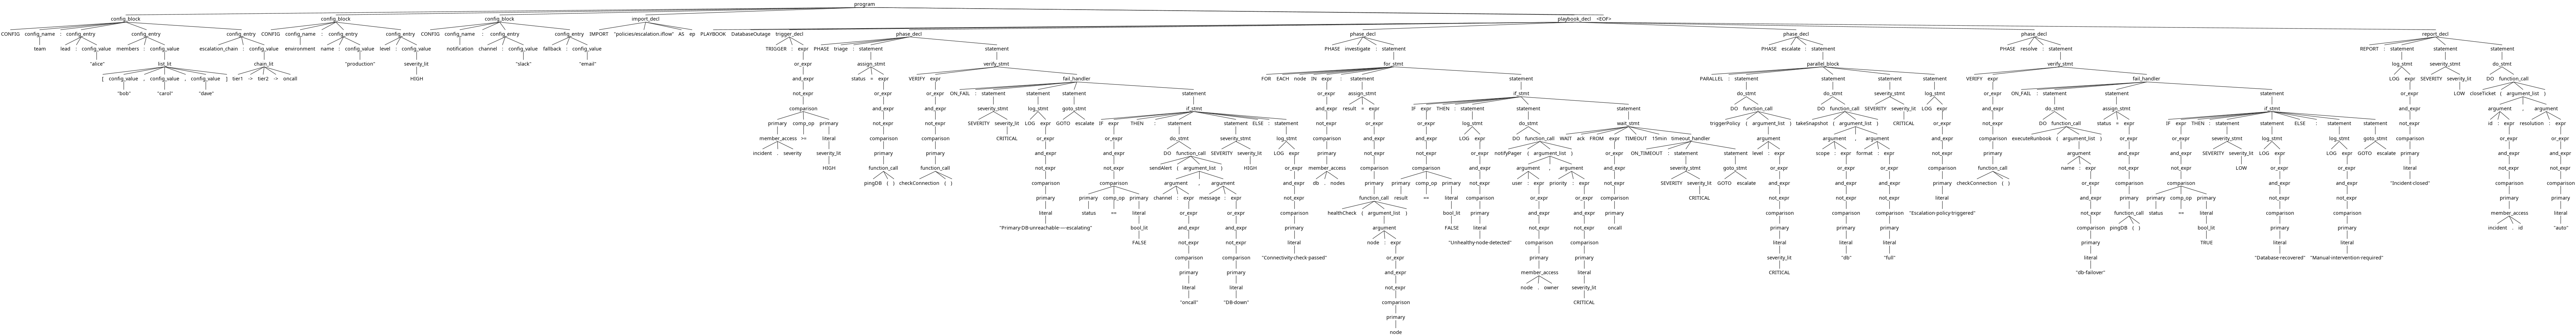
\includegraphics[angle=90,width=1.4\textheight,height=1.4\textwidth,keepaspectratio]{../antlr/antlr4_parse_tree.png}
\end{center}
\clearpage


\section*{A.5 Playbook Sample}

\begin{lstlisting}
CONFIG team:
    lead: "alice"
    members: ["bob", "carol", "dave"]
    escalation_chain: tier1 -> tier2 -> oncall

CONFIG environment:
    name: "production"
    level: HIGH

IMPORT "policies/escalation.iflow" AS ep

PLAYBOOK DatabaseOutage
    TRIGGER: incident.severity >= HIGH

    PHASE triage:
        status = pingDB()
        VERIFY checkConnection()
        ON_FAIL:
            SEVERITY CRITICAL
            LOG "Primary DB unreachable - escalating"
            GOTO escalate

        IF status == FALSE THEN:
            DO sendAlert(channel: "oncall", message: "DB down")
            SEVERITY HIGH
        ELSE:
            LOG "Connectivity check passed"

    PHASE investigate:
        FOR EACH node IN db.nodes:
            result = healthCheck(node: node)
            IF result == FALSE THEN:
                LOG "Unhealthy node detected"
                DO notifyPager(user: node.owner, priority: CRITICAL)

        WAIT ack FROM oncall TIMEOUT 15min
        ON_TIMEOUT:
            SEVERITY CRITICAL
            GOTO escalate

    PHASE escalate:
        PARALLEL:
            DO triggerPolicy(level: CRITICAL)
            DO takeSnapshot(scope: "db", format: "full")
        SEVERITY CRITICAL
        LOG "Escalation policy triggered"

    REPORT:
        LOG "Incident closed"
        SEVERITY LOW
        DO closeTicket(id: incident.id, resolution: "auto")
\end{lstlisting}

\section*{A.6 Problem Map}

\includepdf[pages=-,pagecommand={\thispagestyle{plain}}]{../documentation/T17_PBL_PROBLEM_MAP.pdf}
